\section{Objectifs fonctionnels du programme}

	\subsection{Reconnaissance de caractères}

Le but de projet est de réaliser un programme capable de reconnaitre des
caractères en utilisant un réseau de neurones. Nous tenterons de reconnaitre les
caractères 'a' et 'b'. Cela dit le programme sera général et permettra
d'apprendre à distinguer deux caractères quels qu'ils soient.

Les images seront binaires : elles ne contiennent que deux couleurs: noir et blanc. Cela dit il faut remarquer que l'on ne perd pas en généralité en ne choisissant que des images binaires, en effet un filtre bien sélectionn\'e permettrait de se ramener à une image binaire à partir de n'importe quelle image couleur. L’échantillon d'image sera tiré de plusieurs polices de caractère existantes ainsi que de numérisations de nos écritures à la mains sur les quelles il sera réaliser un filtre afin de se ramener à une image binaire. Le filtre pourra être réalisé très facilement via le logiciel
Gimp.

Les images \`a tester auront pour format 30x30 pixels, mais encore une fois nous ne perdons pas en généralité puisqu'un redimensionnement d'image permettra de convertir n'importe quelle image en se format. Un des premier travail de ce projet sera de réfléchir puis de fixer la façon dont les données de l'image seront communiquées à la couche d'entrée des neurones. En effet on peut envisager plusieurs situation : mettre en entrée les pixels de l'image tels quels ou bien réaliser des prétraitement sur l'image, et donner en enter des données déjà traités.

\begin{center}
	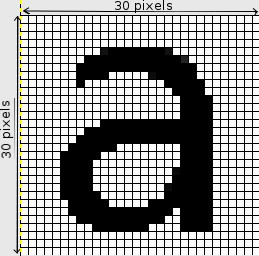
\includegraphics[width=0.66\linewidth]{img/char.png}
\end{center}

La reconnaissance de formes et l'apprentissage dans le domaine de la vision est une application classique des réseaux de neurones, nous pouvons donc espérer réussir à faire marcher , en pratique cette reconnaissance de caractère. De plus nous somme sur de pouvoir trouver de la documentation et de l'aide sur internet puisque ce sujet est assez classique.

	\subsection{Interface du logiciel}

L'interface homme machine du logiciel attendu sera minimaliste et en ligne de
commande. Le logiciel aura deux commandes principales :

\begin{itemize}
	\item \textbf{Lancer la phase d'aprentissage:}	\newline 
%		\textit{neurones -l dossierCarcteres1 dossierCarcteres2[-o neuronesFile]}\newline
		Cette fonctionnalit\'e permettra de r\'ealiser la phase d’apprentissage afin de distinguer les caract\`eres se trouvant sur les images situ\'ees dans un dossier \textit{dossierCaracteres1} de celles situ\'ees dans le dossier \textit{dossierCaracteres2}. Le r\'eseaux de neurones obtenu sera alors stock\'e dans un fichier pour permettre sa r\'eutilisation.
	\item \textbf{Demander une reconnaissance de caract\`ere:} \newline
%		\textit{neurones neuroneFile Limage.bmp}\newline
		L'utilisateur pourra fournir au programme une image. Le programme affichera alors si l'image correspond à un caract\`ere de type 1 ou 2 selon l'apprentissage pr\'ec\'edent.
\end{itemize}